\chapter{Work Plan} \label{chap:workplan}

\section*{}

This chapter describes the general work plan for the thesis, in terms of
activities and their respective timings. Furthermore, we will discuss the
datasets that will be used in the work, their characteristics and provenience.
Lastly, we will address the subject of work evaluation and validation,
explaining how it will be conducted, both during and at the end of the project.

\section{Planning}\label{sec:planning}

Aside the preparation phase (already completed), the time available for the
thesis will span from February to July, 2014, roughly totaling twenty weeks. It
is essential to define a top level schedule beforehand, to ensure that
sufficient time will be allotted for every phase of the project and that the
timings of those phases are feasible. As such, Figure \ref{fig:gantt} represents
the division of the six main phases of the project, during the available period
of twenty weeks. Although each phase comprises several smaller tasks, we believe
that such a small granularity planning is not needed in this phase and will be
defined during the work's execution, as needed. Each main phase of the project
is composed as follows:

\begin{figure}[!ht]
  \begin{center}

    \begin{ganttchart}[
      y unit title=0.6cm,
      y unit chart=0.7cm,
      x unit=0.8cm,
      vgrid,hgrid,
      title height=1,
      bar/.style={fill=gray!50},
      progress label text={},
      bar height=0.4]{12}

      % Time labels
      \gantttitle{2014}{12} \\
      \gantttitle{February}{2}
      \gantttitle{March}{2}
      \gantttitle{April}{2}
      \gantttitle{May}{2}
      \gantttitle{June}{2}
      \gantttitle{July}{2} \\

      % Tasks
      \ganttbar{Information system development}{2}{4} \\
      \ganttbar{Assembly pipeline development}{4}{5} \\
      \ganttbar{Web platform development}{5}{6} \\
      \ganttbar{Transcriptome assembly}{7}{9} \\
      \ganttbar{Transcriptome analysis}{8}{10} \\
      \ganttbar{Thesis writing}{9}{11}
      \ganttbar[bar/.style={fill=gray!20}]{}{2}{8}

    \end{ganttchart}
  \end{center}
  \caption[Work distribution planning]{Work distribution planning.}
  \label{fig:gantt}
\end{figure}

\begin{description}

  \item \textbf{Information system development}
  comprises the design and development of the data management component of the
  project and will take roughly six weeks. Despite not being the most critical
  component, making it the first in the development timeline facilitates later
  data intensive phases like the transcriptome assembly and, at the same time,
  allows extensive testing and performance evaluation through usage. A
  substantial time allotted for this phase will be spent tackling the
  performance aspects of implementing a system for such large quantities of
  data, both in terms of database size and response times.

  \item \textbf{Assembly pipeline development}
  consists of the construction of the tool pipeline responsible for assembling
  the transcriptomes. At first, several of the already mentioned tools will be
  studied and tested against small datasets, in an effort to ascertain which are
  best suited to our particular problem. As the tools are selected, the pipeline
  itself will take shape, integrating the tools in sequence. Any actual
  development effort in this phase will be in the form of simple data format
  conversion scripts, since we will use existing assembly tools. Because of
  this, the estimated duration of this phase is only one month or four weeks,
  despite its critical importance to the project.

  \item \textbf{Web platform development}
  will take four weeks and comprises the design and implementation of the
  system's web front-end. The web platform will integrate the information and
  assembly systems, providing a user friendly interface for genetic data
  storage, management and assembly. From a technical standpoint it's a fairly
  trivial system, which explains why only four weeks were reserved to this
  phase.

  \item \textbf{Transcriptome assembly}
  is the first phase after concluding the development of the main components of
  the system. In this phase the developed system will be used to produce the
  assembled transcriptome, employing the given production dataset. This phase
  will take about six weeks, despite no implementation work taking place (saving
  some small system tweaks). This is because genome and, in this case,
  transcriptome assembly are resource and time intensive processes that can
  take several days, making the extra time necessary for both new and repeat
  experiments.

  \item \textbf{Transcriptome analysis}
  will consist in the usage of several data mining tools in order to try to
  explain the already mentioned RNA transcription mechanisms. This phase is
  expected to last about six weeks. Although not as resource demanding as the
  transcriptome assembly phase, this will require choosing and testing a new
  set of tools and possibly integrate them with the developed system.

  \item \textbf{Thesis writing}
  is the last phase of the project, with an expected six weeks allocated time.
  These last six weeks refer to a period to collect and report the obtained
  results and to make the final reviews to the produced content. However, it is
  expected that the thesis report will be worked on continuously from the start 
  of the project, in parallel with the other project phases.

\end{description}

\section{Experimental Data}\label{sec:datasets}

During this project there will be essentially three types of datasets used: read
data, genome data and test data. Each type of dataset has its own nature, origin
and purpose. We will use real genetic data from a fly species called \fly{},
commonly known as fruit fly, which can be seen in Figure \ref{fig:fly}. It is
one of the most frequently used organisms to provide its genetic data for these
kind of studies and work.

\afterpage{
  \begin{figure}[!htb]
    \begin{center}
      \leavevmode
      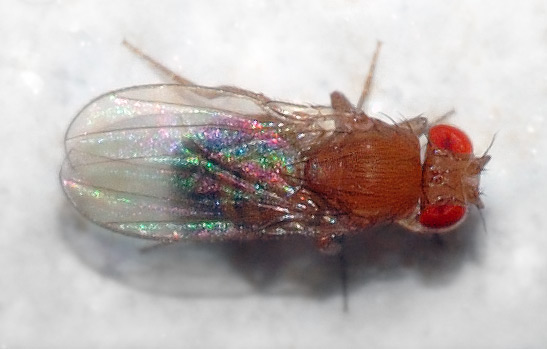
\includegraphics[width=0.6\textwidth]{d_melanogaster}
      \caption[Specimen of \fly]{Specimen of \fly, viewed from above\protect\footnotemark.}
      \label{fig:fly}
    \end{center}
  \end{figure}
  \footnotetext{Image taken from \url{http://pt.wikipedia.org/wiki/Drosophila_melanogaster}.}
}

The read data will be made available during the project through IBMC. As stated,
this data consists of several short sequencing reads of the \fly{} genome. It is
this dataset that will be ultimately used for assembly and posterior data mining
analysis. It should be noted that this will be real data, experimentally
obtained in a laboratory for this project.

The genome data will consist of already assembled \fly{} genome(s), that will be
used as a reference in our own assembly process. This data will be obtained
through FlyBase\footnote{\url{www.flybase.org}}. FlyBase is an online and
publicly accessible database of \Fly{} genes and genomes. This database allows
its data to be downloaded in several formats, that can be either directly used
in our assembly pipeline, or be automatically converted by one of the created
conversion tools.

Lastly, we will use some small scale datasets for the test and calibration of the
assembly pipeline. Such datasets are usually shipped with the assembly tools
themselves. If needed, a combination of the two previous datasets can be used to
produce small scale test data for this purpose.

\section{Thesis Work Evaluation}\label{sec:eval}

In the second part of the project, that is the transcriptome assembly and
analysis phases, results evaluation and validation is essential. Even more so
when such results are typically evaluated from a molecular biology standpoint and
therefore are out of the scope of knowledge of the thesis itself. In such cases
we will have two evaluation methods at our disposal.

The first method is based on relevant metrics and evaluation methods for the
problems at hand, from both the transcriptome assembly and data mining parts. In
the case of transcriptome assembly, we will rely mostly on contextual quality
metrics. These metrics are typically produced by the tools themselves. They
usually have a well defined range of expected results, which makes them a very
important method of early result evaluation, in the sense that they can be
interpreted without a profound knowledge about their molecular biology
foundations. In the case of data mining, we will use the procedures  and
measures described in Section \ref{sec:mineval}.

The second method available is the evaluation by IMBC's technicians, that will
assist us whenever expert biology knowledge is required. This will ultimately be
the method that will provide a real measure of the success of the project.

Furthermore, IMBC's technicians will be essential during the entirety of the project. They
will help steer the project into its intended direction, giving some insight
about their expectations towards the system. Project phases like the
implementation of the information system or the transcriptome analysis will be
driven by their feedback, giving us a sense about what should be done. Lastly,
they will also be present throughout the project to help with any biology
related questions that arise.
